% Options for packages loaded elsewhere
\PassOptionsToPackage{unicode}{hyperref}
\PassOptionsToPackage{hyphens}{url}
%
\documentclass[
]{article}
\usepackage{amsmath,amssymb}
\usepackage{lmodern}
\usepackage{iftex}
\ifPDFTeX
  \usepackage[T1]{fontenc}
  \usepackage[utf8]{inputenc}
  \usepackage{textcomp} % provide euro and other symbols
\else % if luatex or xetex
  \usepackage{unicode-math}
  \defaultfontfeatures{Scale=MatchLowercase}
  \defaultfontfeatures[\rmfamily]{Ligatures=TeX,Scale=1}
\fi
% Use upquote if available, for straight quotes in verbatim environments
\IfFileExists{upquote.sty}{\usepackage{upquote}}{}
\IfFileExists{microtype.sty}{% use microtype if available
  \usepackage[]{microtype}
  \UseMicrotypeSet[protrusion]{basicmath} % disable protrusion for tt fonts
}{}
\makeatletter
\@ifundefined{KOMAClassName}{% if non-KOMA class
  \IfFileExists{parskip.sty}{%
    \usepackage{parskip}
  }{% else
    \setlength{\parindent}{0pt}
    \setlength{\parskip}{6pt plus 2pt minus 1pt}}
}{% if KOMA class
  \KOMAoptions{parskip=half}}
\makeatother
\usepackage{xcolor}
\IfFileExists{xurl.sty}{\usepackage{xurl}}{} % add URL line breaks if available
\IfFileExists{bookmark.sty}{\usepackage{bookmark}}{\usepackage{hyperref}}
\hypersetup{
  pdftitle={Energías Renovables con SmartGrid},
  pdfauthor={Francisco Artero, Ignacio Gambino, Marcos Ander Egg y Justo Roncoroni},
  hidelinks,
  pdfcreator={LaTeX via pandoc}}
\urlstyle{same} % disable monospaced font for URLs
\usepackage[margin=1in]{geometry}
\usepackage{graphicx}
\makeatletter
\def\maxwidth{\ifdim\Gin@nat@width>\linewidth\linewidth\else\Gin@nat@width\fi}
\def\maxheight{\ifdim\Gin@nat@height>\textheight\textheight\else\Gin@nat@height\fi}
\makeatother
% Scale images if necessary, so that they will not overflow the page
% margins by default, and it is still possible to overwrite the defaults
% using explicit options in \includegraphics[width, height, ...]{}
\setkeys{Gin}{width=\maxwidth,height=\maxheight,keepaspectratio}
% Set default figure placement to htbp
\makeatletter
\def\fps@figure{htbp}
\makeatother
\setlength{\emergencystretch}{3em} % prevent overfull lines
\providecommand{\tightlist}{%
  \setlength{\itemsep}{0pt}\setlength{\parskip}{0pt}}
\setcounter{secnumdepth}{-\maxdimen} % remove section numbering
\ifLuaTeX
  \usepackage{selnolig}  % disable illegal ligatures
\fi

\title{Energías Renovables con SmartGrid}
\author{Francisco Artero, Ignacio Gambino, Marcos Ander Egg y Justo
Roncoroni}
\date{2023-10-06}

\begin{document}
\maketitle

\hypertarget{energia-renovables-con-smartgrid}{%
\section{Energia Renovables con
Smartgrid}\label{energia-renovables-con-smartgrid}}

El grado de aproximación a la red inteligente ideal se utiliza para
evaluar las ventajas potenciales que ofrece la integración de fuentes
renovables. La eficiencia de la integración se ha abordado en este
capítulo utilizando una técnica de proceso de jerarquía analítica difusa
que toma en consideración la existencia de varios criterios cualitativos
y cuantitativos, una variedad de indicadores de desempeño y la
imprevisibilidad del entorno de la red inteligente. La elección del
tamaño y la posición de un generador distribuido en el alimentador de
distribución radial sirve como ilustración del proceso.

\hypertarget{introducciuxf3n}{%
\subsection{Introducción}\label{introducciuxf3n}}

La toma de decisiones sobre energías renovables puede verse como un
problema de toma de decisiones con criterios múltiples (MCDM) con
criterios y alternativas relacionados. Debido a la complejidad de
variables sociales, técnicas, ambientales y económicas, esta actividad
debe tener en cuenta una serie de factores opuestos {[}1, 2{]}. La
complejidad de los sistemas modernos y esta cuestión son demasiado para
que las metodologías convencionales de toma de decisiones de criterio
único puedan gestionarlas {[}3, 4{]}. En {[}5, 6{]} se proporciona un
resumen de los modelos y enfoques de vanguardia utilizados para abordar
el problema, evaluando y categorizando las tendencias de investigación
presentes y proyectadas en esta área.

Se han utilizado cinco categorías principales {[}5, 7-13{]} para
clasificar las áreas de aplicación de MCDM en energías renovables:

•Planificación y política de energías renovables, que se refiere a la
evaluación de un plan energético y la difusión de diversas opciones de
energías renovables.

•Evaluación y valoración, que se refiere a la valoración de diversas
energías alternativas o tecnologías energéticas.

•Selección de tecnología y proyectos, que incluye elección de ubicación,
selección de tecnología y apoyo a la toma de decisiones en proyectos de
aprovechamiento de energías renovables; y medioambiental, que se ocupa
de las tecnologías alternativas.

La evaluación de las fuentes renovables ha evolucionado como resultado
del desarrollo del diseño de redes inteligentes, trayendo consigo nuevas
metas y objetivos. Una red energética que tiene la capacidad de integrar
de forma inteligente las actividades de cada usuario conectado a ella
para ofrecer de forma eficaz un suministro eléctrico seguro, asequible y
sostenible se conoce como ``red inteligente''. Las tecnologías de
comunicación bidireccional y procesamiento informático que se han
utilizado durante años en otros sectores son las que permiten estos
sistemas. Los principales objetivos de las redes inteligentes, según
{[}14{]}, son mejorar el uso de fuentes de electricidad renovables,
asegurar el sistema, promover la eficiencia y conservación de la energía
y crear un mercado energético desregulado. Por lo tanto, la estrategia
para una energía competitiva, sostenible y segura implica principalmente
competitividad, el uso de diversas fuentes de energía, sostenibilidad,
innovación y avance tecnológico {[}15{]}, mientras que se deben evaluar
los beneficios potenciales de la integración de fuentes renovables. por
el grado de aproximación a la red inteligente ideal.

Se han establecido tres marcos de evaluación principales en el contexto
de la red inteligente. Las cualidades de las redes inteligentes ideales
(servicios) y los resultados de la implementación de la red inteligente
ideal han sido presentados por el Grupo de trabajo de la CE sobre redes
inteligentes {[}16, 17{]}.

A través de un conjunto de indicadores clave de desempeño (KPI), la
contribución de las iniciativas a la red inteligente ideal se cuantifica
en términos de beneficios. El sistema de red inteligente ideal ha sido
separado en áreas temáticas (clústeres) por la Iniciativa Europea de Red
Eléctrica {[}18{]}, y este mapeo de proyectos en grupos está actualmente
en marcha. En los Estados Unidos se han establecido los atributos
ideales y un conjunto de métricas para medir el progreso hacia redes
inteligentes ideales {[}19{]}: construir métricas que describan las
características que se construyen en apoyo de una red inteligente (por
ejemplo, la proporción de subestaciones que utilizan automatización ) y
métricas de valor o impacto que describen los beneficios potenciales de
lograr una red inteligente (por ejemplo, porcentaje de energía consumida
para generar electricidad que no se pierde, o cantidad de electricidad
entregada a los consumidores en comparación con la electricidad generada
expresada como porcentaje).

El estudio propone un algoritmo novedoso para la evaluación de la
integración de fuentes de energía renovables en la red inteligente, que
utiliza el método del proceso de jerarquía analítica difusa (AHP) para
la toma de decisiones multicriterio. Esto se debe a la proliferación de
criterios tanto cuantitativos como cualitativos, así como a muchas
incertidumbres relacionadas con el entorno de operación de las redes
inteligentes. Saaty creó el primer AHP a finales de los años 1970
{[}20{]}. Los juicios humanos se representan de esta manera como valores
nítidos. Sin embargo, el modelo de preferencia humana es incierto en
muchas situaciones del mundo real, lo que dificulta que los responsables
de la toma de decisiones proporcionen valores numéricos precisos a las
evaluaciones comparativas. En estas situaciones se debe utilizar el
enfoque AHP difuso. La técnica difusa AHP tiene como objetivo mejorar el
apoyo a las decisiones para prioridades y valores ambiguos. La técnica
de este artículo utiliza preferencias de expertos y datos evaluados en
un contexto de conjunto difuso {[}21{]}. La incorporación de información
no cuantificable, información incompleta, información inalcanzable y
conocimiento parcialmente desinformado en modelos de decisión es posible
gracias a la aplicación de la teoría de conjuntos difusos {[}22{]}.

Numerosos autores han aplicado el método AHP difuso a una variedad de
cuestiones, incluida la gestión de los recursos hídricos {[}23, 24{]},
la evaluación de sistemas de misiles tácticos navales {[}25-28{]}, la
gestión de residuos peligrosos {[}29{]}, la priorización de indicadores
de medición del capital humano {[}30{]}, la gestión de activos marítimos
{[}31{]} y la gestión de la seguridad laboral {[}32, 33{]}. Hay varios
casos en los que se utiliza AHP difuso en la industria de las energías
renovables, con ejemplos que incluyen la asignación de recursos
renovables {[}37, 38{]}, el estudio económico de la eficiencia de las
tecnologías renovables {[}36{]} y la priorización de tecnologías
energéticas {[}4, 34, 35{]}. Debido a las numerosas ventajas y criterios
ambiguos e intangibles que intervienen en la evaluación de proyectos de
redes inteligentes, en esta investigación se emplea la técnica difusa
AHP para evaluar y elegir proyectos de redes inteligentes.

Desarrollamos una metodología de evaluación novedosa para evaluar la
integración de fuentes renovables en una red inteligente, trabajando a
partir de un amplio conjunto de métricas de desempeño de la red
inteligente. El enfoque descrito en esta investigación identifica el
conjunto ideal de actividades relacionadas con las energías renovables
en la segunda etapa basándose en una coincidencia difusa de
alternativas. Validamos nuestra técnica en una red de prueba y
demostramos que es bastante eficaz para evaluar alternativas cuando
existen varios conjuntos de criterios en competencia.

La técnica difusa AHP se presenta después de una breve descripción de
métricas de rendimiento importantes para la evaluación de redes
inteligentes. El enfoque se demuestra seleccionando una de las cuatro
opciones de inserción de generador distribuido para el alimentador de
distribución radial de prueba de 33 barras IEEE, cada una con un tamaño,
ubicación y tecnología diferentes. A continuación se proporcionan las
conclusiones sobre la idoneidad de la técnica sugerida, junto con
recomendaciones para futuras investigaciones.

\hypertarget{marcos-de-evaluaciuxf3n-de-redes-inteligentes}{%
\subsection{Marcos de evaluación de redes
inteligentes}\label{marcos-de-evaluaciuxf3n-de-redes-inteligentes}}

Los objetivos de política estratégica, como la integración fluida de las
fuentes de energía renovables, un suministro de energía más confiable y
sostenible y la plena participación de los consumidores en el mercado de
la electricidad, pueden lograrse con la ayuda de la implementación de
una red inteligente. La red eléctrica puede controlarse con tolerancias
considerablemente más estrictas para los servicios públicos gracias a un
mejor conocimiento de su estado segundo a segundo, lo que conduce a una
mayor confiabilidad y eficiencia.

Dirigir la transición a las redes inteligentes es una tarea difícil y
prolongada que requiere lograr un equilibrio entre los objetivos de
política energética, los límites ambientales y la viabilidad comercial.
En consecuencia, un primer paso para evaluar la ``red inteligente
ideal'' y sus resultados previstos (como la sostenibilidad, la
eficiencia y la inclusión de los consumidores), que están directamente
relacionados con los objetivos políticos que han desencadenado esta
transición, es evaluar en qué medida Los proyectos de energía renovable
están avanzando en este objetivo. Para llevar a cabo esta primera
estrategia se utiliza la definición de mediciones adecuadas y de
desempeño crítico. Una segunda estrategia complementaria implica el uso
de una metodología adecuada de análisis de decisiones multicriterio para
evaluar la viabilidad financiera de las soluciones e inversiones de
energía renovable integradas en la red inteligente. Las siguientes
secciones aclararán ambos pasos.

\hypertarget{muxe9tricas-de-evaluaciuxf3n-de-redes-inteligentes}{%
\subsubsection{Métricas de evaluación de redes
inteligentes}\label{muxe9tricas-de-evaluaciuxf3n-de-redes-inteligentes}}

En {[}17-19, 39{]} se exponen las características de las mejores redes
inteligentes y los criterios utilizados para evaluar los resultados de
la implementación de estos proyectos. La red inteligente ideal ha sido
descrita en términos de ``características'' en los Estados Unidos y en
términos de ``servicios'' en la Unión Europea, incluyendo:

•Permitir que la red integre a los usuarios con nuevos requisitos.

•Mejorar la eficiencia del funcionamiento diario de la red.

•Permitir una mejor planificación de futuras inversiones en redes.

•Garantizar la seguridad de la red, el control del sistema y la calidad
del suministro.

•Permitir y promover una mayor y más directa participación de los
consumidores en su consumo y gestión de energía.

Para cada servicio se han definido una serie de funcionalidades
relevantes de redes inteligentes.

Las mediciones de valor/construcción se utilizan en los Estados Unidos
para medir el progreso hacia la red ideal, mientras que los
beneficios/KPI se emplean en Europa.

El Grupo de Trabajo sobre Redes Inteligentes de la CE ha elaborado una
lista de ventajas resultantes de la adopción de una red inteligente
{[}17{]}, que incluye •Mayor sostenibilidad.

•Conexión y acceso a la red adecuados para todo tipo de usuarios de la
red.

•Niveles adecuados de seguridad y calidad del suministro.

•Mayor eficiencia y mejor funcionamiento de la red.

•Capacidad adecuada de las redes de transmisión y distribución para
``recolectar'' y llevar electricidad a los consumidores.

•Apoyo efectivo a los mercados eléctricos transnacionales mediante el
control del flujo de carga para aliviar los flujos en bucle y aumentar
las capacidades de interconexión.

•Mayor conocimiento del consumidor y participación en el mercado por
parte de nuevas empresas.

•Permitir a los clientes tomar decisiones fundamentadas sobre su energía
para alcanzar los objetivos de eficiencia energética de la UE.

•Desarrollo coordinado de la red a través de una planificación
compartida de la red europea, regional y local.

•Establecer un mecanismo de mercado para nuevos servicios energéticos
para los consumidores, como la eficiencia energética o la consultoría
energética.

•Reducir o reducir la presión sobre los crecientes costos de consumo.

Se utiliza una colección de KPI con indicadores cuantitativos y
cualitativos para expresar cada beneficio. A modo de ejemplo, el primer
beneficio, una mayor sostenibilidad, se mide por la disminución
cuantificada de las emisiones de carbono, el efecto ambiental de la
infraestructura que sustenta la red eléctrica y la disminución
cuantificada de los accidentes y los riesgos resultantes del uso de
tecnologías de generación. En {[}17{]} hay una lista completa de todos
los indicadores. La sostenibilidad, la competitividad y la seguridad del
suministro son los objetivos políticos que impulsan el despliegue de la
red inteligente y, como resultado, los servicios y beneficios de la red
inteligente pueden considerarse métricas útiles para evaluar la
contribución de los proyectos al cumplimiento de estas políticas.
objetivos.

Un marco bien establecido puede mostrar con precisión cómo un proyecto
contribuye a un sistema eléctrico inteligente. En términos de proyectos
de energía renovable, se puede crear una lista ajustada de criterios
clave, que incluyen:

•Comience con la lista de servicios clave y beneficios asociados para
obtener una comprensión completa del estado del desarrollo de las redes
inteligentes. Ventajas financieras (FB): opciones de precios al
consumidor, menores costos unitarios de producción y costos
estabilizados.

•Conservación de energía y beneficios ambientales (ECEB): reducción de
gases de efecto invernadero y otros contaminantes, reducción de la
generación de energía a partir de fuentes no económicas mediante la
mejora del uso de FER.

•Beneficios de la energía eficiente (EEB): uso óptimo de la energía,
reducción de las pérdidas de energía, gestión de la demanda durante los
picos y posibilidad de operar el sistema eléctrico con la máxima
eficiencia a través de la gestión de la energía.

•Los beneficios para la seguridad y la protección (SSB) incluyen una
mejor comprensión de las condiciones riesgosas o peligrosas, una mejor
seguridad física y cibernética del sistema y protección de la
privacidad.

El segundo conjunto de indicadores de desempeño en el nivel base de
evaluación de la eficiencia de la integración de energías renovables se
seleccionó de la lista completa de indicadores después de especificar el
primer nivel de beneficios. La disminución mensurable de las emisiones
de carbono, el desempeño de la calidad del voltaje de las redes
eléctricas (como las caídas de voltaje, las desviaciones de voltaje y
frecuencia, y la cantidad de pérdidas en las redes de distribución, ya
sean pérdidas absolutas o porcentuales), y estos son los indicadores que
pueden ser monitoreado. El valor actual neto de la inversión podrá
incrementarse mediante la evaluación de nuevas iniciativas. Las ventajas
sociales y los efectos ambientales evaluados del proyecto sirven como
indicadores cualitativos.

Una de las principales justificaciones para la introducción de enfoques
MCDM es la combinación de datos cuantitativos y cualitativos. Otro
factor son las deficiencias del análisis costo-beneficio, que se
analizarán con más detalle en la siguiente sección.

\hypertarget{modelo-de-evaluaciuxf3n-multicriterio}{%
\subsubsection{Modelo de evaluación
multicriterio}\label{modelo-de-evaluaciuxf3n-multicriterio}}

El mercado debería verificar cómo se implementa la red inteligente. Por
lo tanto, evaluar los costos, ventajas y beneficios de diversas
soluciones es otro paso crucial en el proceso de evaluación de redes
inteligentes. La Comisión Europea ha desarrollado y modificado el
enfoque DOE/EPRI para adaptarse al entorno europeo {[}41, 42{]},
mientras que se ha creado una metodología completa para el análisis
costo-beneficio de estos proyectos {[}40{]}.

Pero cuando se trata de estrategias de desarrollo, cuando los factores
intangibles no son sólo secundarios sino que en realidad ocupan un lugar
central, la técnica convencional de análisis de costo-beneficio se queda
corta {[}43{]}. La conversión de todos los impactos en una única medida
numérica agregada es el principal inconveniente del análisis
costo-beneficio. Por lo tanto, parece que el análisis de criterios
múltiples, que emplea más de un criterio y introduce componentes
cualitativos al estudio, es mejor para cuantificar intangibles y efectos
secundarios que el análisis de costo-beneficio.

Se crea un modelo de criterios múltiples utilizando la lista de
indicadores cuantitativos y cualitativos que figuran en las Secciones.
5.2.2.1. y 5.2.2.2, como se indica en la Sección. 5.2.1.

\hypertarget{indicadores-cuantitativos}{%
\paragraph{Indicadores Cuantitativos}\label{indicadores-cuantitativos}}

En esta metodología se utiliza un conjunto de cuatro indicadores
cuantitativos:

•Reducción cuantificada de emisiones de carbono Esta métrica se calcula
para cada alternativa en base a los kilogramos de emisiones de CO2 por
kilovatio-hora de energía eléctrica producida. La disminución de las
emisiones producidas por las fuentes de energía tradicionales se
considera impacto de las fuentes de energía renovables. La desviación de
voltaje total se calcula usando la ecuación. (5.1):

\(V_D = \sqrt {\sum_{k=1}^{NB} (V_k - V_{ref})^2}\)

donde Vk es la magnitud del voltaje en la barra k, Vref es la magnitud
del voltaje flojo de la barra y NB es el número total de nodos en la
red.

•Las pérdidas de potencia activa se calculan como:

\(P_{loss}=\sum_{j=1}^{NL}i^2_jR_j\)

donde Rj e ij son la resistencia y la corriente real de la j-ésima
línea, respectivamente, y NL es el número total de líneas.

•El total descontado de todos los flujos de efectivo recibidos del
proyecto se utiliza para calcular el valor presente neto (VAN), que se
utiliza para evaluar el valor presente de una inversión. El cálculo de
la suma descontada de todos los flujos de efectivo se puede reescribir
como:

\(NPV=\sum_{j=1}^{NL}C_i (1+d)^i - C_0\)

donde C0 es la inversión inicial, Ci es el flujo de caja, d es la tasa
de descuento y n es el período de tiempo.

\begin{figure}
\centering
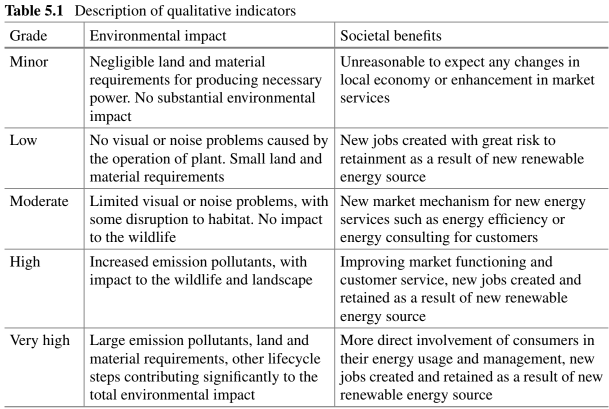
\includegraphics{fotos/tabla5.1.png}
\caption{tabla 1}
\end{figure}

\hypertarget{indicadores-cuanlitativos}{%
\paragraph{Indicadores cuanlitativos}\label{indicadores-cuanlitativos}}

El beneficio social (SB) de una inversión en infraestructura propuesta y
el efecto ambiental (EI) de la infraestructura de la red energética son
métricas no exactas que se evalúan mediante comparación ordinal. En esta
estrategia, utilizamos la escala verbal de cinco grados para evaluar
estos indicadores, que pueden estar compuestos por resultados de
encuestas de opinión, opiniones profesionales u otras estrategias
integradas. La tabla 5.1 proporciona una explicación de la escala.

Todos los indicadores (cualitativos y cuantitativos) tienen efectos
variables sobre los cuatro criterios básicos, dependiendo de quién toma
las decisiones. Por ejemplo, un perfil de voltaje estable y una menor
variación de voltaje en la red permitirían el uso de servicios y
tecnología de vanguardia al tiempo que reducirían los gastos asociados
con la mala calidad de la energía y aumentarían la satisfacción del
cliente. La Figura 5.1 ilustra la jerarquía de niveles y relaciones
entre criterio, subcriterio y alternativas.

\hypertarget{muxe9todo-de-evaluaciuxf3n-de-redes-inteligentes}{%
\subsection{Método de evaluación de redes
inteligentes}\label{muxe9todo-de-evaluaciuxf3n-de-redes-inteligentes}}

La evaluación de la integración de fuentes renovables en la red
inteligente se realiza en esta investigación utilizando el enfoque
difuso AHP. Los conjuntos difusos, los números difusos y la aritmética
difusa proporcionan la base de las matemáticas del método AHP difuso.

\begin{figure}
\centering
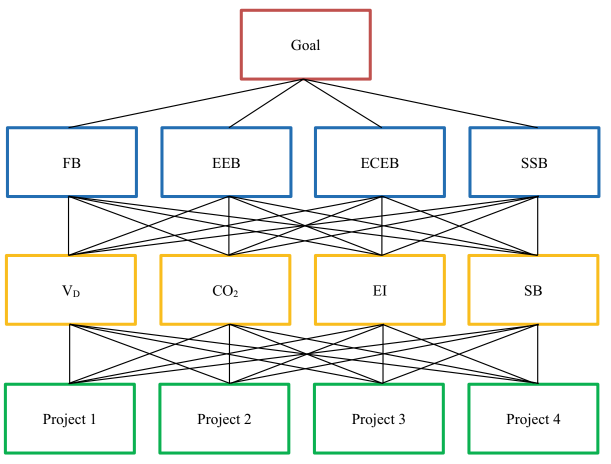
\includegraphics{fotos/foto_diagrama.png}
\caption{figura 1}
\end{figure}

\hypertarget{conjuntos-difusos-nuxfameros-difusos-triangulares-y-aritmuxe9tica-difusa}{%
\subsubsection{Conjuntos difusos, números difusos triangulares y
aritmética
difusa}\label{conjuntos-difusos-nuxfameros-difusos-triangulares-y-aritmuxe9tica-difusa}}

Zadeh define un conjunto difuso A por grado de membresía \(µ_{A}(x)\)
sobre un universo de discurso X como {[}44{]}:

\(µ_{A}(x):X \rightarrow [0,1]\)

Un número difuso es un conjunto difuso convexo y normalizado
A=\{(x,\(µ_{A}(x)\)),x ∈ R.

Un número difuso triangular se puede denotar como M=(a,b,c), y la
función de membresía es:

\[
\mu_{A(x)} = \begin{cases}
\frac{-a}{b} & \text{si } x \in [a, b] \\
\frac{c - x}{c - b} & \text{si } x \in [b, c] \\
0 & \text{en otro caso}
\end{cases}
\]

donde \$ a\leq b \leq c\$, a y c representan los valores inferior y
superior del apoyo de M superior, respectivamente, y bis el valor modal.
Cuando \(a=b=c\), es un número nítido.

La aritmética difusa se basa en el principio de extensión de Zadeh.Si
\(f:X \rightarrow Y\) es una función y A es un conjunto difuso en X,
entonces \(f(A)\) esta definida como:

\(\mu_{f(A)y} = \sup_{x \in X} \mu_{f(A)y}\)

donde \(y ∈ Y\)

Leyes básicas del número difuso triangular \(M=(a,b,c), a>0\), son:

\(M^{-1}=(a,b,c)^{-1}=(\frac{1}{c},\frac{1}{b},\frac{1}{a})\)

\(M^n=(a,b,c)^n=(a^n,b^n,c^n), n∈N\)

\(M^{\frac{1}{n}}=(a,b,c)^\frac{1}{n}=\)

Las principales leyes de las operaciones con dos números difusos
triangulares \(M_1(a_1,b_1,c_1)\) y \(M_2(a_1,b_1,c_1)\) son:

•Suma de números difusos:

\(\text{M1} \oplus \text{M2} = (a_1, b_1, c_1) \oplus (a_2, b_2, c_2) = (a_1 + a_2, b_1 + b_2, c_1 + c_2)\)

•Resta de números difusos:

\(M_1θM_2=(a_1, b_1, c_1)θ(a_2, b_2, c_2)=(a_1-c_2,b_1-b_2,c_1-a_2)\)

•Multiplicación de números difusos:

\(M_1⊙M_2=(a_1, b_1, c_1)⊙(a_2, b_2, c_2)=(a_1 *a_2, b_1 * b_2, c_1 * c_2),a_1,a_2>0\)

•División de números difusos:

\(M_1∅M_2=(a_1, b_1, c_1)∅(a_2, b_2, c_2)=(\frac{a_1}{c_2},\frac{b_1}{b_2},\frac{c_1}{a_2}),a_1,a_2>0\)

\hypertarget{muxe9todo-ahp-difuso}{%
\subsubsection{Método AHP difuso}\label{muxe9todo-ahp-difuso}}

Los siguientes pasos están involucrados en el método AHP difuso:

Paso 1: Identificar y establecer claramente el objetivo general
(objetivo).

Paso 2: Identificar los criterios, subcriterios y alternativas.

Paso 3. La formación de la estructura jerárquica.

Paso 4: Comparación por pares utilizando la escala de evaluación difusa
de Saaty.

Paso 5: Evaluación del método de media geométrica de filas (RGMM) de los
vectores de ponderación de prioridad.

Paso 6: El índice de consistencia geométrica (GCI) se utiliza para
determinar si las evaluaciones son consistentes.

Paso 7: Se clasifican las alternativas y se define la defusificación.
Las siguientes fases están incluidas en el proceso de siete pasos del
algoritmo difuso AHP para evaluar fuentes de energía renovables:

•Estableciendo una meta. El objetivo es evaluar la eficacia con la que
las plantas de energía renovable se integran en el entorno de las redes
inteligentes.

•Determinación de los criterios, subcriterios y alternativas. Las
ventajas financieras, los beneficios del uso eficiente de la energía,
los beneficios de la conservación de la energía y el medio ambiente, y
los beneficios de la seguridad son todos criterios de selección para las
iniciativas de redes inteligentes. Los KPI son subcriterios, como se
describe en las Secciones. 5.2.2.1. y 5.2.2.2. Como alternativas, se
enumeran otros proyectos que integran energías renovables.

•La creación de estructuras jerárquicas. La técnica AHP difusa plantea
un problema en forma de estructura jerárquica, con el objetivo en la
parte superior, los criterios relevantes en el segundo nivel (cuatro
criterios identificados), los subcriterios relevantes en el tercer nivel
(cuatro KPI identificados) y las opciones renovables en el segundo
nivel. el cuarto nivel (cuatro alternativas).

•Comparación por pares. Utilizando la escala difusa de Saaty, se
comparan pares de ítems en cada nivel de acuerdo con su contribución
relativa a los componentes en el nivel jerárquico anterior, como se
ilustra en la Tabla 5.2. Se utilizan números difusos triangulares para
implementar la fusificación en este estudio y {[}27{]} recomienda
utilizar un valor de distancia difusa de 2 para obtener resultados más
confiables.

Las comparaciones por pares en cada nivel, comenzando desde la parte
superior de la jerarquía, se presentan en forma de matriz cuadrada
\(A=[a_{ij}]_{i,j=1,n}\) donde \(a_{ij}\) es el valor difuso sobre la
importancia relativa de los criterios/subcriterios/alternativa i sobre
los criterios/subcriterios/alternativa j, \(a_{ij}=1\) para i=j y
\(a_{ij}*a_{ij}=1\) para \(i=j\)

•Evaluación de vectores ponderados prioritarios. El RGMM se utiliza para
evaluar los vectores de ponderación de prioridad en cada nivel. La
selección del vector de ponderación de criterios inicia el proceso de
clasificación:

\begin{figure}
\centering
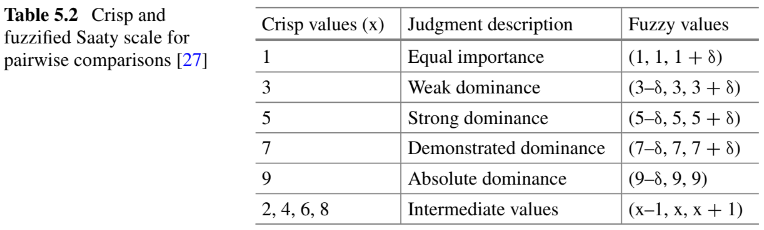
\includegraphics{fotos/tabla 5.2.png}
\caption{figura 2}
\end{figure}

\(W_c=(w_{c1},w_{c2},w_{c3},w_{c4})^T\),

donde \(w_{c1}\) es el peso difuso del \(i\)-ésimo criterio:

\(w_{ci}=\frac{(\prod_{j=1}^{4}a_{ij})^{\frac{1}{4}}}{\sum_{i=1}^{4}(\prod_{j=1}^{4}a_{ij})^{\frac{1}{4}}}, i=\overline{1,4}\)

Mediante la comparación por pares de indicadores de desempeño para cada
criterio, se crean vectores de ponderación de subcriterios. Los
componentes apropiados de estos vectores se determinan de la siguiente
manera:

\(w_{sci}^{p}=\frac{(\prod_{j=1}^{4}a_{ij})^{\frac{1}{4}}}{\sum_{i=1}^{4}(\prod_{j=1}^{4}a_{ij})^{\frac{1}{4}}}, i=\overline{1,4}\)
, \(p=\overline{1,4}\)

donde \(w_{sci}^{p}\) representa el peso difuso del i-ésimo indicador de
desempeño con respecto al \(p\)-ésimo criterio. El vector de ponderación
de subcriterios final se obtiene multiplicando la matriz de
ponderaciones de subcriterios según todos los criterios (\(W_1\)) y la
matriz de ponderaciones de criterios (\(W_c\)):
\(W_a=W_2\otimes W_{sc}=(w_{a1},w_{a2},w_{a3},w_{a4})^{T}\)

\begin{itemize}
\tightlist
\item
  Control de consistencia.
\end{itemize}

Al comparar criterios, subcriterios o alternativas, la coherencia se
refiere a la capacidad del procedimiento de decisión para proporcionar
conclusiones que tengan sentido. Cuando se emplea el RGMM como
procedimiento de priorización, el GCI se utiliza para el control de
coherencia {[}21, 45, 46{]}. Para una matriz de juicio \(n \times n\),
el GCI se calcula de la siguiente manera:

\(GCI=\frac{2}{(n-1)(n-2)}\sum_{i\lt j}^{}log^{2}e_{ij}\),

donde\(e_{ij}=a_{ij}w_j/w_i\) es el error obtenido cuando la relación
\(w_i/w_j\) se aproxima mediante
\(a_{ij} , i, j = 1, n (a_{ij} , w_i , w_j\) son valores de
defusificación, es decir, valores nítidos). Para esta medida, los
umbrales asociados con el nivel de inconsistencia del 10\% sugerido por
Saaty son GCI = 0,31 para n = 3, GCI = 0,35 para n = 4, GCI = 0,37 para
n \textgreater{} 4 {[}47,48{]}.

\begin{itemize}
\tightlist
\item
  Defusificación y clasificación alternativa al final.
\end{itemize}

En este estudio, se utiliza el enfoque del valor medio para clasificar
números difusos triangulares. Para el número difuso triangular dado
\(M = (a,b,c)\), el método del valor medio para la desdifusificación es
un valor numérico nítido definido de la siguiente manera:

\(m=\frac{a+b+c}{3}\),

El rango más alto tiene la alternativa con el valor más alto de m.

\hypertarget{resultados-y-discusiuxf3n}{%
\subsection{Resultados y discusión}\label{resultados-y-discusiuxf3n}}

La tecnología elegida, el tamaño y la ubicación de un generador
renovable distribuido sirven como ejemplos de la técnica sugerida. En el
alimentador de prueba radial IEEE de 33 barras (Fig. 5.2), se evalúan
cuatro posibles soluciones utilizando la potencia activa nominal (Pnom),
el nodo al que está conectado el generador (Bus N°), el tipo de fuente
renovable (RS) y la producción de energía anual prevista del generador
(W), como se muestra en la Tabla 5.3.

Valores tanto para indicadores cualitativos como cuantitativos, tal y
como se explica en los Apartados 5.2.2.1. y 5.2.2.2, se representan en
la Tabla 5.4.

Los expertos primero realizan una comparación por pares de los
siguientes criterios: beneficios financieros (\(C_1\)), beneficios
energéticos eficientes (\(C_2\)), conservación de energía y beneficios
ambientales (\(C_3\)) y beneficios de seguridad (\(C_4\)). Los
resultados de la comparación, pesos difusos, pesos crujientes y rangos
de criterios se muestran en la Tabla 5.5.
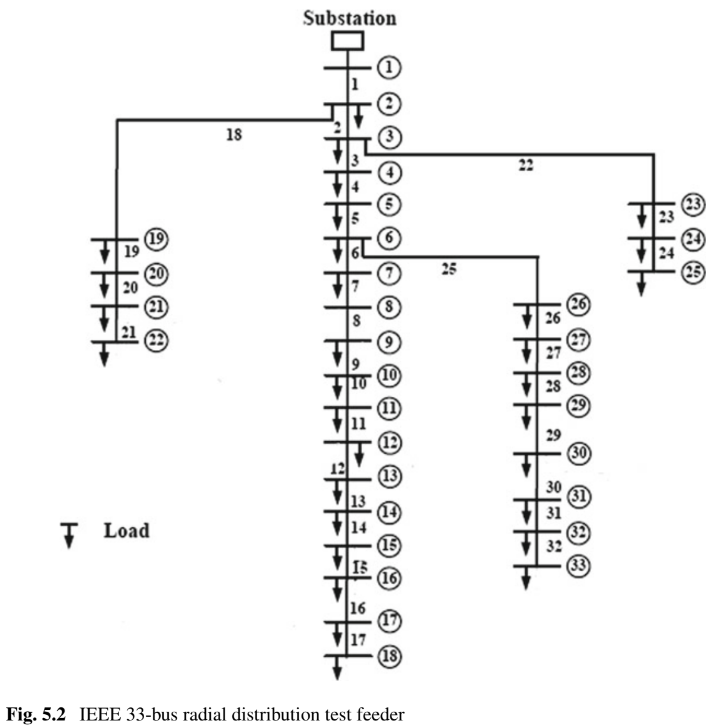
\includegraphics{fotos/foto2.png} 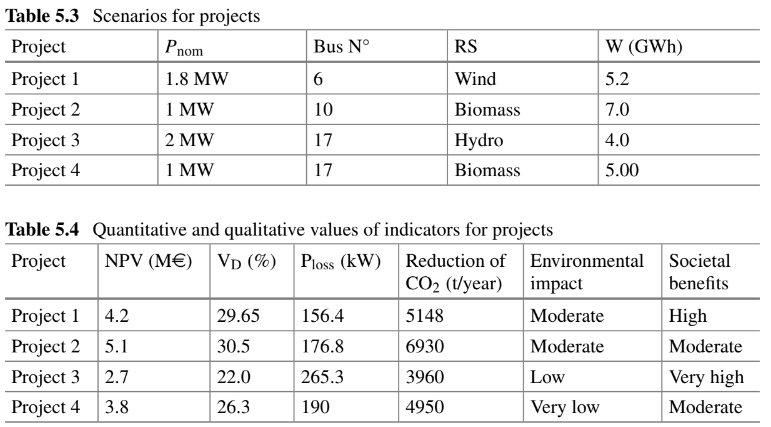
\includegraphics{fotos/tabla5.png}
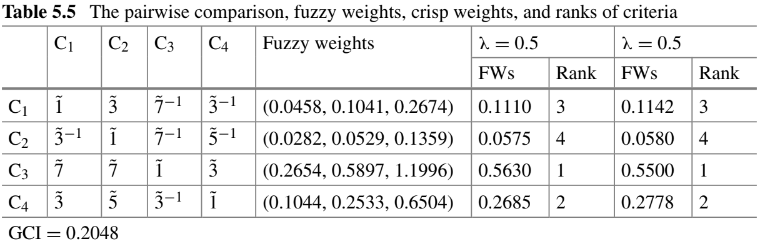
\includegraphics{fotos/tabla5.5.png}

Luego, los expertos comparan los siguientes indicadores clave de
desempeño en relación con cada criterio: desviación de voltaje
(\(SC_1\)), reducción de emisiones (\(SC_2\)), impacto ambiental
(\(SC_3\)) y beneficios sociales (\(SC_4\)). Los resultados se presentan
en las Tablas 5.6, 5.7, 5.8 y 5.9.

Los pesos difusos finales de los KPI, según la ecuación. (5.18) y los
Cuadros 5.5, 5.6, 5.7, 5.8 y 5.9, son:

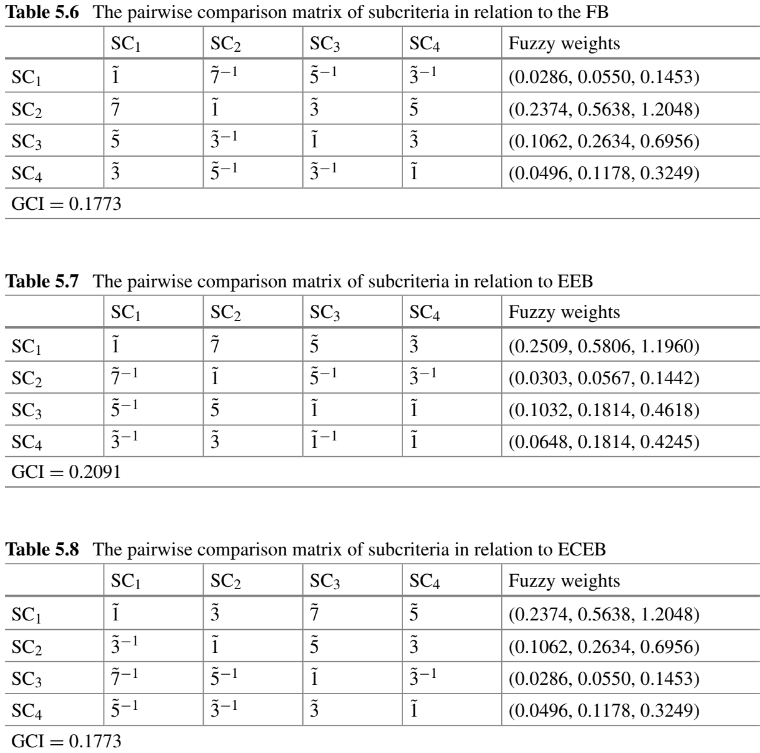
\includegraphics{fotos/tabla5.8.png}
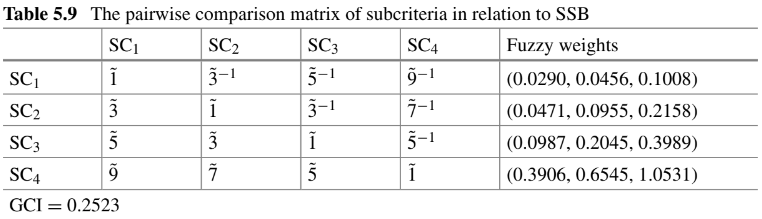
\includegraphics{fotos/tabla5.9.png}

\[W_{sc}=\begin{bmatrix}(0.0744, 0.3805, 1.7122)\\ (0.0448, 0.2412, 1.3166)\\ (0.0580, 0.2571, 1.2193)\end{bmatrix} \]

Al final, se comparan cuatro proyectos de redes inteligentes (Proyecto 1
{[}\(A_1\){]}, Proyecto 2 {[}\(A_2\){]}, Proyecto 3 {[}\(A_3\){]} y
Proyecto 4 {[}\(A_4\){]}) en relación con los KPI presentados en las
Tablas 5.3 y 5.4 tal como se presentan en Tabla 5.10.

Los pesos difusos finales para proyectos de redes inteligentes, según la
Ec. (5.19) y los resultados de la comparación por pares de alternativas
en relación con todos los KPI calculados a partir de los valores dados
en la Tabla 5.10, son:

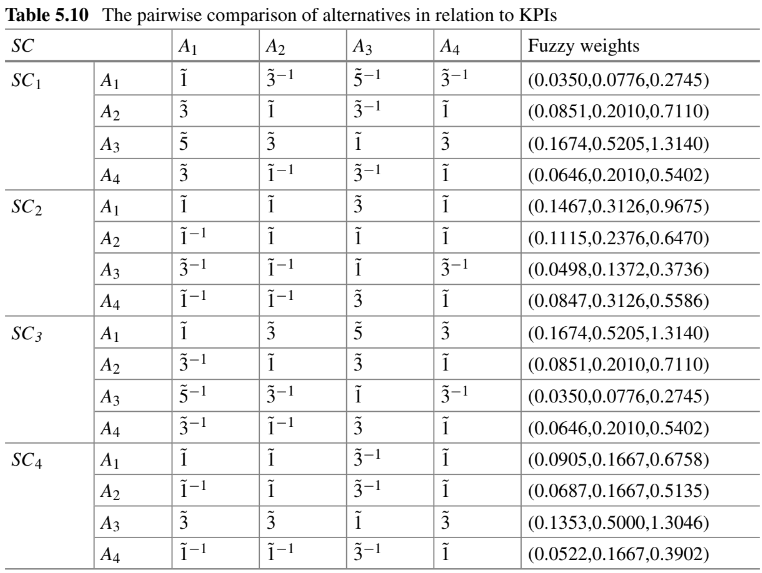
\includegraphics{fotos/tabla5.10.png}
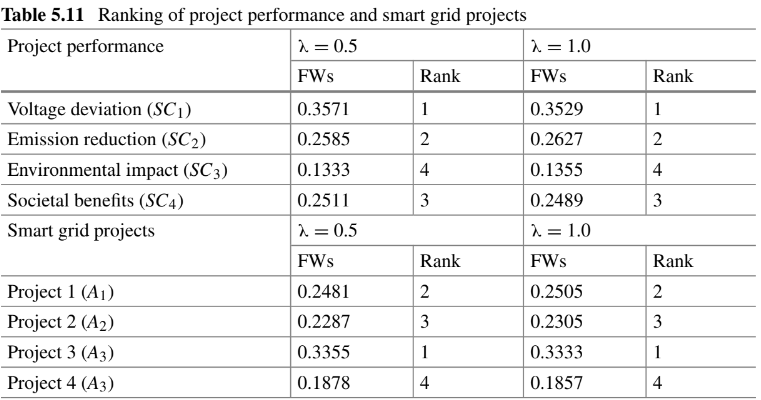
\includegraphics{fotos/tabla5.11.png} \$W\_\{a\}=

\begin{bmatrix}(0.0187, 0.2109, 3,4646)\\  (0.0175, 0.2412, 3.3166)\\   (0.0234, 0.2571, 4.5193)\\(0.0133, 0.2157, 2.5048)\end{bmatrix}

\$

Los proyectos de rendimiento y de redes inteligentes se clasifican tras
la desdifusificación de los vectores de ponderaciones finales de
rendimiento y proyectos. La Tabla 5.11 muestra las clasificaciones (los
FW son ponderaciones finales).

Con base en los resultados anteriores podemos concluir lo siguiente:

\begin{itemize}
\item
  La conservación de energía y los beneficios ambientales ocupan el
  primer lugar entre los criterios de selección para un proyecto basado
  en la efectividad de la integración de plantas de energía renovable en
  el contexto de una red inteligente, seguidos por los beneficios de
  seguridad, los beneficios financieros y los beneficios del uso
  eficiente de la energía.
\item
  El principal indicador de desempeño para las ventajas financieras es
  la reducción de emisiones, seguido de los beneficios del uso eficiente
  de la energía, la conservación de la energía y el medio ambiente, la
  variación de voltaje y los beneficios sociales para la seguridad.
\item
  Estas son las clasificaciones finales de los KPI, teniendo en cuenta
  todos los factores: (1) desviación de voltaje; (2) reducción de
  emisiones; (3) beneficios sociales; y (4) efecto ambiental.
\item
  Según la clasificación final de los proyectos, el Proyecto 3 ocupa el
  puesto más alto, seguido de los Proyectos 1, 2 y 4, teniendo el
  Proyecto 4 la prioridad más baja.
\end{itemize}

Esto indica que se debe elegir el Proyecto 3 para el despliegue de la
red inteligente.

\hypertarget{conclusiuxf3n}{%
\subsection{Conclusión}\label{conclusiuxf3n}}

El nuevo método para evaluar la efectividad de los proyectos de energía
renovable es determinar cuánto avanzan la ``red inteligente ideal'' y
sus resultados anticipados (por ejemplo, sostenibilidad, eficiencia e
inclusión del consumidor).

En este capítulo se emplea el enfoque AHP difuso para brindar apoyo a
las decisiones sobre valores y prioridades inciertos. Se ha ideado una
nueva metodología de evaluación de la integración de fuentes renovables
en la red inteligente, partiendo de un amplio conjunto de indicadores de
rendimiento de la red inteligente. El enfoque descrito en esta
investigación estima la distribución ideal de los recursos de energía
renovable basándose en una coincidencia difusa de alternativas.

La técnica sugerida se demuestra seleccionando el mejor tamaño,
ubicación y tecnología para la integración anticipada de recursos
renovables en la red de distribución actual. Demostramos el excelente
desempeño del método en la evaluación de alternativas frente a diversos
criterios utilizando cuatro criterios principales y seis subcriterios
generados a partir del conjunto seleccionado de ventajas de la red
inteligente. Esta técnica permite a los tomadores de decisiones incluir
información incompleta, poco confiable, no cuantificable y parcialmente
desinformada en el modelo de decisión.

\textbf{Agradecimientos} Este trabajo fue apoyado por el Ministerio de
Educación, Ciencia y Desarrollo Tecnológico de Serbia a través del
Instituto de Matemáticas de la Academia de Ciencias y Artes de Serbia.

\end{document}
